\chapter{Anforderungsanalyse}
\label{chap:anforderungsanalyse}
    Dieses Kapitel befasst sich im Allgemeinen mit der Anforderungsanalyse und -erhebung. Hierbei wird eine
    Marktanalyse repräsentiert, um das Potential rundum \acl{SH} aufzuzeigen und ein Gefühl 
    dafür zu vermitteln, welche Anforderungen dabei entstehen können, bzw. bereits bestehen. Die Analyse ist 
    mit repräsentativen Statistiken, Studien und Umfragen belegt. Hauptsächlich wird im Rahmen der Anforderungserhebung 
    auf die Methodiken und Techniken eingegangen, die verwendet werden, um 
    Anforderungen zu identifizieren. Diese dienen als Grundlage für die Konzeption der Steuerzentrale. Bestandteile der 
    Anforderungserhebung sind unter anderem zentrale Prozesse des \acl{RE}, ein \textit{user-centered Design}, im Deutschen 
    nutzerzentriertes Design, eine \textit{Target Group Analysis}, im Deutschen Zielgruppenanalyse, und die Durchführung von 
    Experten Interviews. Diese Interviews sind nicht repräsentativ und dienen lediglich der weiträumigeren Informationsgewinnung. 
    \\
    Vorab wird sichergestellt, dass im Rahmen des benutzerzentrierten Designs der Softwareentwickler als Nutzer und Anwender im 
    Vordergrund steht, da dieser die Plattform betreibt, bzw. für die Erweiterung der Software als auch für die 
    Anpassungen auf die eigenen Anwendungsfälle zuständig ist.
    \\
    \linebreak
    Damit ein Eindruck entsteht, welches Marktpotential \acl{SH} Anwendungen haben und welche Anforderungen somit 
    verbunden sind, wird basierend auf gegebenen Studien, Statistiken und Umfragen eine Marktanalyse durchgeführt.

\section{Marktanalyse}
\label{sec:marktanalyse}
    Der Markt rundum \acl{SH} nimmt immer weiter zu. Sei es die Entwicklung von neuen intelligenten Geräten, die 
    Massentauglichkeit von Geräten %, die nicht lange am Markt bestehen 
    oder die stetig wachsende Abdeckung von Anwendungsfällen und Übernahme von Aufgaben und Prozessen. Durch die Vielzahl an 
    Produktanbietern und diversen Kommunikationsmöglichkeiten, ist es schwierig eine Lösung für alle Alternativen und 
    Produktausprägungen anzubieten. Hersteller versuchen mit der angebotenen Produktpalette ihr eigenes Ökosystem im Bereich 
    \acl{SH} zu erstellen, um die Nutzer abhängig zu machen. Der repräsentativen Studie von Deloitte zufolge ist jedoch eine 
    Insellösung bei den Nutzern in Deutschland nicht gefragt \cite{deloitte2018}. Befragt wurden 2000 Konsumenten zwischen 
    19 und 75 Jahren. Einem geringen Anteil von 22 Prozent der 
    Befragten ist die Erweiterbarkeit des Systems mit Produkten anderer Hersteller weniger, bzw. nicht wichtig. Im Gegensatz dazu 
    empfinden 43 Prozent der Befragten die Erweiterbarkeit als wichtig und 28 Prozent als sehr wichtig \cite{deloitte2018}. 
    Demnach müssen die Hersteller eine flexiblere Einsetzbarkeit gewährleisten, damit solche Systeme den Marktdurchbruch 
    erlangen. Dadurch wird die Entwicklung von Plattformen komplexer und umfangreicher. Beispielsweise sind die am weit 
    verbreitetsten Open Source Plattformen, openHAB und Home Assistant, sehr komplex und bilden ein großes Ökosystem ab, da 
    stetig der Zuwachs an integrierbaren Geräten zunimmt und damit der Funktionsumfang steigt.  

    \subsection{Allgemeine Marktsituation und Marktprognose}
    %Anbieter, Plattformen, Geräte
        Derzeit gibt es viele Anbieter für intelligente Produkte. Diese bieten zum einen einzelne Geräte an, die in 
        beliebige Plattformen integriert werden können und zum anderen ein eigenes Ökosystem, sofern der Anwender 
        mehrere Produkte des Anbieters nutzen möchte. Dennoch ist in den meisten Fällen die Konfiguration der Geräte nur auf 
        den hauseigenen Plattformen möglich. Somit kann der Nutzer nicht alle Komponenten ausschließlich über eine Plattform 
        konfigurieren und steuern. 
        \\
        \linebreak
        Eine repräsentative Umfrage der \ac{SGCS} mit 1384 Teilnehmern, welche im April 2022 veröffentlicht wurde, zeigt, welche 
        Anbieter in Deutschland am meist verbreitetsten sind, bzw. welche die Nutzer am häufigsten kaufen. An oberster Stelle 
        steht Philips und Samsung mit jeweils 25 Prozent und an dritter Stelle Bosch mit 23 Prozent. Weitere Anbieter können dem 
        Diagramm im Anhang (siehe \ref{appendix:brandings}) entnommen werden. Dabei sind jedoch weitaus nicht alle Hersteller und 
        Anbieter aufgelistet. Detaillierter wird an dieser Stelle jedoch nicht eingegangen. 
        \\
        \linebreak
        Der aktuelle Markt für intelligente Produkte ist in sechs primäre Segmente aufgeteilt, die jeweils andere Anwendungsfälle 
        abdecken \cite{statista2021}:
        \begin{itemize}
            \item Kontrolle und Konnektivität: Gateways die alle Geräte jeglicher Segmente kontrollieren, intelligente Lautsprecher 
            mit dem Fokus zur Kontrolle und der digitalen Unterstützung und bspw. intelligente Steckdosen
            \item Intelligente Geräte (Smart Appliances): Kühlschrank, Waschmaschine und Geschirrspüler, Kaffeemaschine, Mikrowelle 
            und Staubsaugerroboter
            \item Sicherheit: Bewegungs-, Wasser- und Rauchmelder, Kameras und Türschlösser
            \item Heimunterhaltung (Home Entertainment): Fernseher, Entertainment-Systeme 
            \item Komfort und Licht: Intelligente LEDs, Fenster- und Tür-Sensoren etc.
            \item Energiemanagement: Thermostate und Regler, Luftqualitätsmesser etc. 
        \end{itemize}
        \pagebreak
        Die aufgelisteten Segmente werden von vielen Herstellern bedient. Darunter sind der folgenden Abbildung die 
        repräsentativen Schlüsselanbieter zu entnehmen:
        \begin{figure}[hbt!]
            \centering
            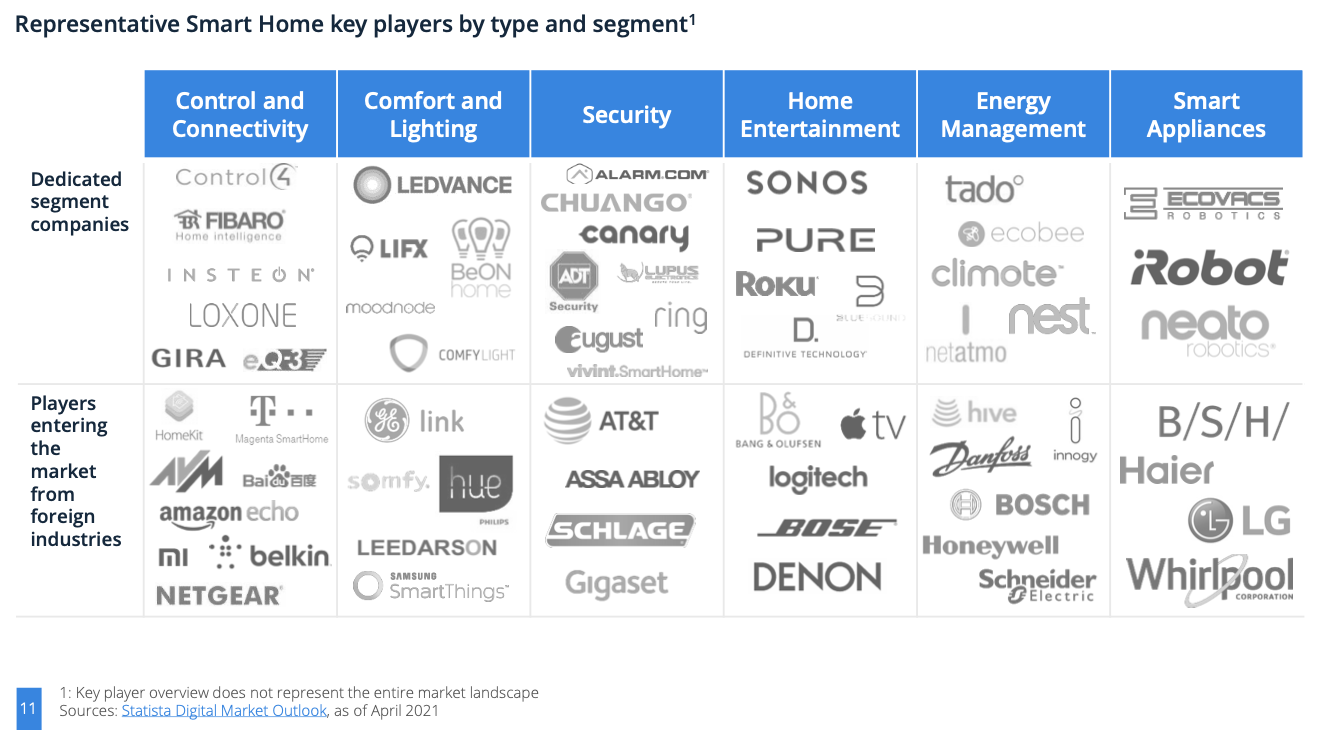
\includegraphics[width=15cm,height=10cm,keepaspectratio]{images/keyplayers.png}
            \caption{Übersicht der repräsentativen Schlüsselanbieter \cite{statista2021}} 
            \label{pic:landscape}
        \end{figure}
        \\
        Die Übersicht deckt jedoch nicht alle Anbieter ab und spezialisiert sich in diesem Fall auf die bekanntesten und die am 
        Markt etablierten. 
        \\
        \linebreak
        Laut den von Statista veröffentlichten Daten war die USA mit einem Umsatz von 28,86 Milliarden US-Dollar der größte 
        \acl{SH} Markt im Jahr 2021, wogegen Deutschland eine Umsatz von 6,59 Milliarden US-Dollar erzielte. Zu berücksichtigen sind 
        dabei jedoch die Demographische Lage als auch die Bevölkerungsdichte. Diese Aufstellung steht in keinem direkten Vergleich und 
        dient lediglich zur Veranschaulichung und zur Unterscheidung der Marktanteile. Deutlich wird dabei jedoch, dass das 
        Marktwachstum prozentual ähnlich ansteigt. 
        \\
        \linebreak
        Der Markt-Prognose in Abbildung (\ref{pic:revenue}) ist zu entnehmen, dass bis 2026 sich der Umsatz nahezu verdoppeln 
        wird. Der Darstellung (\ref{pic:globalmarket}) der einzelnen Segmente kann entnommen werden, dass der Weltmarkt von 
        2021 bis 2026 um ca. 100 Prozent zunimmt. Die Zeitspanne von 2019 bis 2026 stellt einen durchschnittlichen Zuwachs von 
        17,4 Prozent dar. Anhand der Prognose und des Berichts von Statista ist deutlich zu sehen, dass der \acl{SH} Markt in 
        den nächsten Jahren erheblich wachsen wird. Prognostiziert ist ein globaler Marktwert bei ca. 207,8 Milliarden 
        US-Dollar bis 2026.
        \begin{figure}[hbt!]
            \centering
            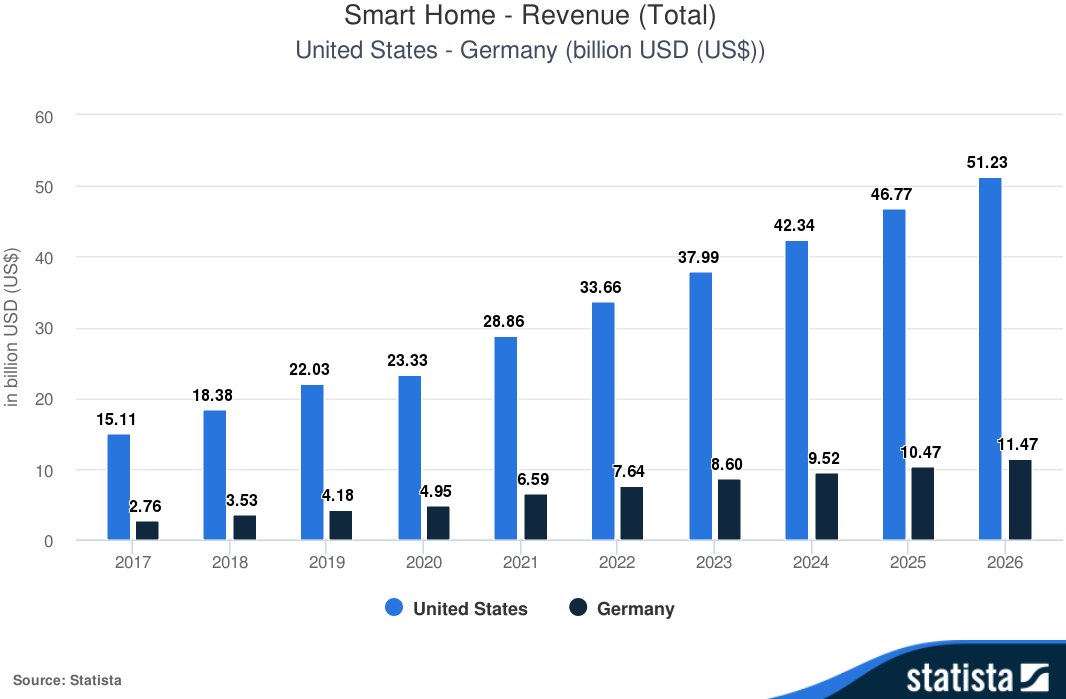
\includegraphics[width=15cm,height=9.25cm,keepaspectratio]{images/Statista-Outlook-Smart-Home---Revenue-Total-United-States---Germany-billion-USD-US.png}
            \caption{Umsatz-Prognose von Deutschland und den USA \cite{statista2021}} 
            \label{pic:revenue}
        \end{figure}
        \\
        \begin{figure}[hbt!]
            \centering
            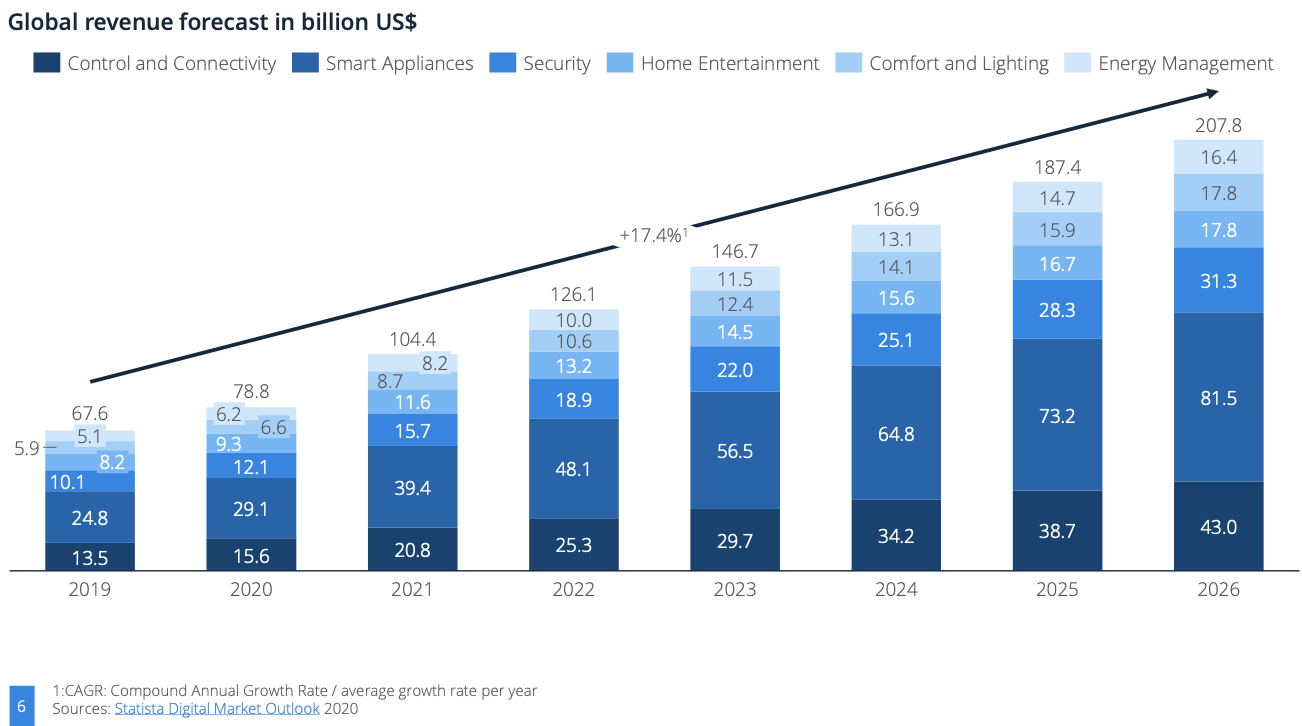
\includegraphics[width=15cm,height=10cm,keepaspectratio]{images/global_Worth_smart-home.png}
            \caption{Globaler Smart Home Marktwert \cite{statista2021}} 
            \label{pic:globalmarket}
        \end{figure}
        \pagebreak 
    \subsection*{Schlüsseltechnologien und Barrieren}
        Unter den Schlüsseltechnologien im \acl{SH} sind Komponenten zu verstehen, die den Gedanken eines intelligenten 
        Wohnraumes und Gebäudes forcieren. Dazu zählen unter anderem die Spracherkennung, die bei Sprachassistenten, 
        darunter bspw. Amazon Alexa, Apple HomePod (Siri) und dem Google Nest, eingesetzt wird, sowie \ac{AI} und \ac{KI} 
        zur Analyse, Auswertung und Optimierung von Verhaltensmustern und weiteren Analysezwecken \cite{statista2021}. 
        Obwohl die Spracherkennung das Wachstum des Marktes ankurbelt, werden die herkömmlichen Interaktionsmöglichkeiten, 
        z.B. die Kontrolle über Berührung durch Touch-Displays,
        weiter bestehen und weiterhin eine wichtige Art des Gerätezugriffs darstellen \cite{all-electronics2022}. 
        Mit dem Einsatz von \acs{KI} und \acs{AI} werden Prozesse noch autonomer und können den Komfort aus den Analysen je 
        nach Bedürfnis individuell gestalten. Zu berücksichtigen ist dabei jedoch die dafür geeigneten Anwendungsfälle und 
        die Bereitschaft der Nutzer, in wie fern diese das Analysieren von Verhaltensmustern akzeptieren und zulassen. 
            
        \subsubsection*{Fehlender Interoperabilität}
            Die Kommunikation von \acl{SH} Geräten findet über drahtlose Netzwerke auf Brandbreiten statt, die oft nicht 
            miteinander kompatibel sind. Der hauptsächliche Grund dafür ist, dass Unternehmen ein Protokoll für einen 
            bestimmten Zweck entwickeln und dieses darauf abgestimmt ist den Anwendungsfall abzudecken und um eine 
            Markteintrittsbarriere zu schaffen, sodass der Wechsel zwischen Anbietern erschwert wird \cite{statista2021}. 
            Die damit einhergehende Schwachstelle eines \acl{SH} ist, dass die Geräte mit den bereits entwickelten 
            Protokollen genutzt werden. So ist die Kommunikation über verschiedene Protokollen nicht vorgesehen. Dadurch 
            entsteht die fehlende Interoperabilität, die der Anwender jedoch für eine \acl{SH} Lösung ansieht und auch 
            als äußerst sinnvoll betrachtet. Die Einführung von Bluetooth LE Mesh ist eine aktuelle Entwicklung, um der 
            Herausforderung der Bewältigung der Interoperabilität einen Schritt näher zu kommen. Dennoch muss der 
            Anwender prüfen, welche Geräte miteinander kompatibel sind \cite{statista2021}. Bei cloudbasierten 
            Sprachdiensten muss ebenso die Kompatibilität geprüft werden. 
            Dadurch wird dem Nutzer neben der Ungewissheit der Datensicherheit und der Privatsphäre ein weiterer Aspekt 
            geliefert, der die Nutzung von \acl{SH} Lösungen für bestimmte Anwendergruppen immer noch in Frage stellt.
            \\ 
            \linebreak
            Derzeit häufig verwendete Protokolle sind unter anderem Bluetooth, \ac{WLAN} (WiFi), KNX, ZigBee, Z-Wave, 
            MQTT und weitere (siehe \ref{tab:protocolsSH}). Um Beispielsweise mit ZigBee über \acs{MQTT} kommunizieren zu 
            können, gibt es ein Framework, welches die Interoperabilität der beiden Protokolle ermöglicht. Dies ist das 
            sogenannte \textit{ZigBee2MQTT} Framework\footnote{Erschafft eine Brücke zwischen ZigBEE und MQTT. \url{https://www.zigbee2mqtt.io/} Abgerufen am 23.05.2022}.
\pagebreak
\section{Zielgruppenanalyse}
\label{sec:zielgruppenanalyse}
    Zur Analyse der Zielgruppen, die \acl{SH} Lösungen nutzen, bzw. die als Anwender des im Rahmen dieser Arbeit 
    entstehenden Konzeptes gelten, erfolgt in diesem Abschnitt eine Zielgruppenanalyse. Hierbei wird zwischen 
    zwei Gruppen stark differenziert. Zum einen erfolgt die Benutzer-Analyse, die aufzeigt, welche Zielgruppen 
    im allgemeinen Kontext \acl{SH} adressiert werden, und zum anderen die Anwender-Analyse, die sich 
    konkret der Zielgruppe widmet, die in dieser Arbeit adressiert wird. 

    \subsection{Ziel der Zielgruppenanalyse}
        %was soll damit erzielt werden?
        Ziel einer Zielgruppenanalyse\footnote{Beschreibung der Zielgruppenanalyse und mögliche Durchführungsschritte. \url{https://www.eology.net/magazine/target-group-analysis} Abgerufen am 24.05.2022.} 
        ist die Identifizierung der Personengruppen, die als potentielle Nutzer eines Produktes 
        oder eines Marktsegmentes gelten. Diese Methodik ist ein relevantes Werkzeug in der Produktkonzeption und -entwicklung 
        als auch in der Marktforschung. Maßnahmen und Anforderungen können aus der Zielgruppenanalyse abgeleitet und 
        erarbeitet werden. 
        \\
        Ein Weiteres Ziel ist das bessere Kennenlernen der Zielgruppe, um dadurch deren Bedürfnisse und Interessen 
        genauer zu identifizieren und zu betrachten. 
    
        \subsection{Benutzer-Zielgruppe}
        % Smart Home - Deutschland. Zugriff: 11. Mai 2022. https://de.statista.com/outlook/dmo/smart-home/deutschland
            Die in der Marktanalyse (\ref{sec:marktanalyse}) identifizierten Segmente werden in der Abbildung 
            (\ref{pic:segments}) nochmals aufgegriffen. Hierbei wird in der repräsentativen Statistik und Prognose der 
            Statista GmbH die Nutzung des jeweiligen Segments veranschaulicht. Der Fokus dieser Prognose liegt 
            auf der verstärkten Vertretung eines Segments in einem \acl{SH} in Deutschland. Die derzeit am meisten eingesetzten 
            Segmente sind \textit{Vernetzung und Steuerung} (rot gekennzeichnet) und \textit{Komfort und Licht} 
            (gelb gekennzeichnet). Das am wenigsten genutzt Segment stellt die \textit{Gebäudesicherheit} 
            (schwarz gekennzeichnet) in der Prognose dar. Im Jahr 2021 lag die Nutzung von Geräten des Segments \textit{Vernetzung 
            und Steuerung} bei 6,6 Millionen Nutzer, dicht gefolgt von dem Segment \textit{Komfort und Licht} mit 
            6,5 Millionen Nutzer. Dagegen liegt das Segment \textit{Home Entertainment} im Jahr 2021 bei 3,8 Millionen Nutzer.
            \\
            \linebreak
            Die bis 2026 veröffentlichte Prognose gibt vor, dass die jeweiligen Segmente stark zunehmen %werden 
            und sich jeweils vervierfachen.  
            \pagebreak
            \begin{figure}[hbt!]
                \centering
                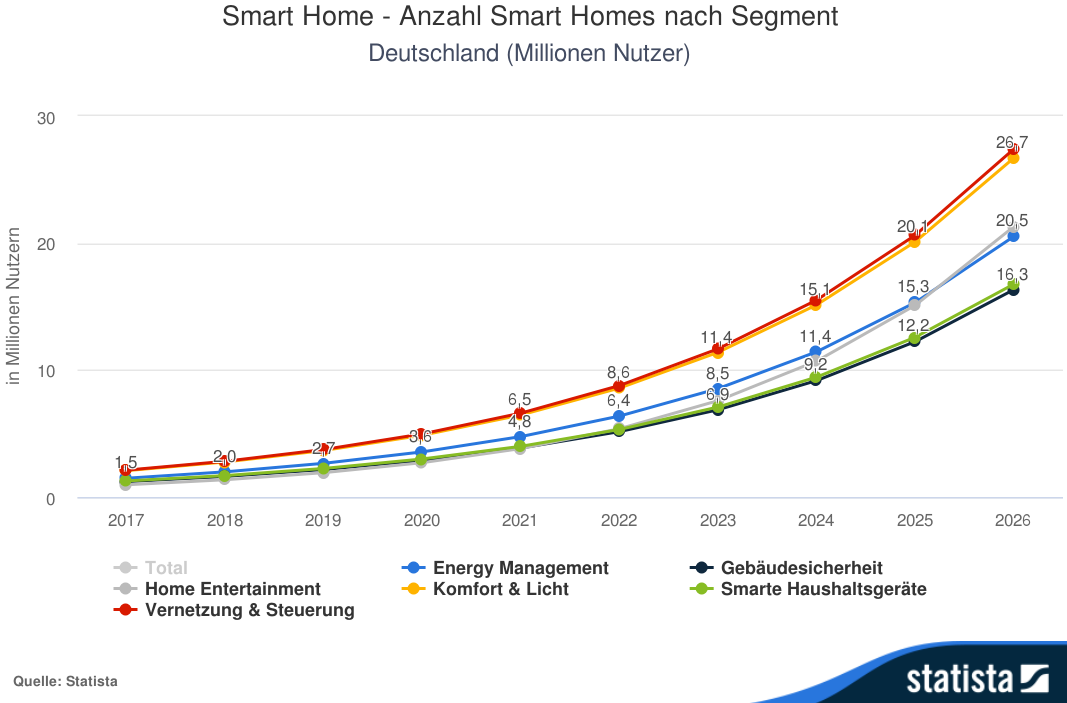
\includegraphics[width=15cm,height=10cm,keepaspectratio]{images/Statista-Outlook-Smart-Home---Anzahl-Smart-Homes-nach-Segment-Deutschland-Millionen-Nutzer.png}
                \caption{Anzahl Smart Home nach Segment \cite{statista2021}} 
                \label{pic:segments}
            \end{figure}
            \\
            Das Resümee der Prognose zeigt, dass eine breitere Masse an Personen bereits Komponenten der Segmente 
            \textit{Vernetzung und Steuerung} und \textit{Komfort und Licht} nutzen.
            \\
            \linebreak
            Im Hinblick auf die demographischen Statistiken wird in der Zielgruppenanalyse deutlich, welche Gesellschaftsschicht 
            im Jahr 2021 am stärksten vertreten ist. Diese erstreckt sich über eine Altersspanne von 25 bis 54 Jahren. 
            Wobei der Abbildung (\ref{pic:ageSH}) zu entnehmen ist, dass der Schwerpunkte im Alter zwischen 45 und 54 Jahren 
            mit 22,7 Prozent. Die Balance nach Geschlecht liegt bei einem Anteil von 45,6 Prozent weiblichen Befragten und 
            54,4 Prozent männlichen Befragten, demnach eine geringe Ungleichheit. Die Auswertung nach Einkommen zeigt, dass 
            35,4 Prozent der Befragten mit mittlerem Einkommen Komponenten eines \acl{SH} nutzen, dicht gefolgt von 
            Personen mit hohem Einkommen, diese liegen bei 34,9 Prozent. 
            \\
            \linebreak
            Demzufolge ist eine große Masse adressiert, die jedoch nach den Segmenten (siehe Abbildung \ref{pic:segments}) 
            wiederum eingeschränkt werden kann.
            \begin{figure}[hbt!]
                \centering
                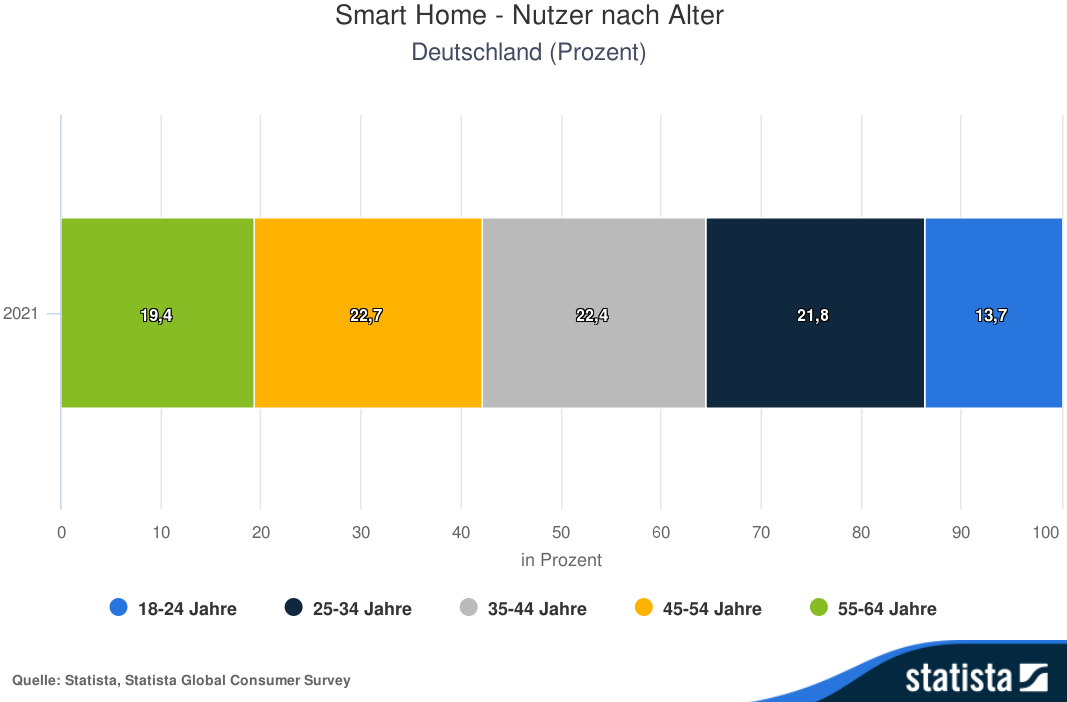
\includegraphics[width=15cm,height=10cm,keepaspectratio]{images/Statista-Outlook-Smart-Home---Nutzer-nach-Alter-Deutschland-Prozent.png}
                \caption{Smart Home Nutzer nach Alter \cite{statista2021}} 
                \label{pic:ageSH}
            \end{figure}
            Die aufgeführten Statistiken und Prognosen zeigen den Markt rundum \acl{SH} auf und welches Potential für die 
            nächsten Jahre prognostiziert wird. Im Hinblick auf die Zielgruppe lässt sich sagen, dass eine breite Masse 
            fokussiert werden kann, die jeweils unterschiedliche Voraussetzungen und Bedürfnisse haben. Diese Analyse zeigt 
            jedoch den gesamten Markt auf, um einen Einblick zu gewährleisten, wie stark \acl{SH} momentan in Deutschland, den 
            Vereinigten Staaten (USA) und dem Rest der Welt vertreten ist. Um einen konkreteren Einblick 
            zu gelangen, wird in nachfolgendem Abschnitt auf die Zielgruppe der Anwender, die in dieser Arbeit fokussiert werden, 
            eingegangen. 

        \subsection{Anwender-Zielgruppe}
            %Die eigentliche Zielgruppe, die
        %Softwareentwickler, die das System betreiben und für ihre Bedürfnisse anpassen.

\section{Use Cases}
\label{sec:usecases}
    Für die Erhebung und Ausarbeitung aller Anforderungen an das System, werden Anwendungsfälle, sogenannte Use Cases, 
    definiert, bewertet und auf ihre Funktionalität geprüft und dokumentiert. Zum besseren Verständnis wird auf diese in den 
    folgenden Abschnitten eingegangen. 
\subsection{Check in mit Temi}
\subsection{Notfallevakuierung mit Temi}
\section{Experten Interview}
\label{sec:experteninterviewReqirements}
    %Die Experten Interviews sind eine Möglichkeit, die Anforderungen zu erfassen, die durch die Entwicklung des Systems 
    %nicht durch eine einfache Marktanalyse erfasst werden konnten. Diese Interviews sind nicht repräsentativ und dienen lediglich 
    %der weiträumigeren Informationsgewinnung.
\subsection{Ziele des Experten Interviews}
\subsection{Aufbau des Experten Interviews}
\subsection{Zusammenfassung der Experten Interviews}
    % Aus den Interviews ergaben sich Anforderungen, die in die Konzeption mit einfließen. Diese werden im folgenden 
    % Abschnitt thematisiert.
\section{Anforderungen}
